\documentclass{scrartcl}

\usepackage[ngerman]{babel}
\usepackage[utf8]{inputenc}
\usepackage[hidelinks]{hyperref}
\usepackage{graphicx}

\begin{document}
	\title{CodeCamp: Context Awareness, Entwicklung einer Android-App}
	\author{Adrian Kunz, Jan Bingemann, Johann Feser, Michael Prasil, Sven Starcke}
	\date{Kassel, den \today}
	
	\maketitle
	\newpage
	
	\tableofcontents
	\newpage
	
	\section{Einleitung}
		\paragraph*{Ziele}
		Ziel des Projektes war es, im Rahmen der Veranstaltung \glqq Code Camp 1: Context Awareness\grqq{} eine Android-basierte Anwendung zur Verwaltung und Aufzeichnung der Einkäufe, welche in der ComTec-Küche getätigt werden, zu erstellen.
		
		\paragraph*{Funktionsweise}
		Auf Basis einer Datenbank können Gegenstände angelegt, gekauft und gelöscht werden. Ein dazu benötigter Nutzer wird ebenfalls in der Datenbank gespeichert. Der Zugriff auf die Datenbank erfolgt über eine REST-API, welche alle notwendigen Operationen bereitstellt.
		
		\paragraph*{Inhalt}
		In Abschnitt ~\ref{features} werden die von der App bereitgestellten Features vorgestellt. Abschnitt ~\ref{architecture} erklärt die Anwendungsstruktur aus technischer Sicht, jeweils für Datenmodell (Abschnitt ~\ref{architecture.datamodel}), die Oberflächen-Architektur (Abschnitt ~\ref{architecture.frontend}) und die zugrunde liegende Grundstruktur inklusive Netzwerkverkehr (Abschnitt ~\ref{architecture.backend}).
		
	\section{Features} \label{features}
	
	\section{Architektur} \label{architecture}
		\subsection{Datenmodell} \label{architecture.datamodel}
			\paragraph*{}
			Das Datenmodell umfasst drei Klassen: \texttt{Item}, \texttt{User}, \texttt{Purchase}. Die Klassen sind passend zur bereitgestellten Datenbank implementiert und haben die in Abbildung ~\ref{datamodel} gezeigte Struktur.
		
		\begin{figure}[!h]
			\label{datamodel}
			%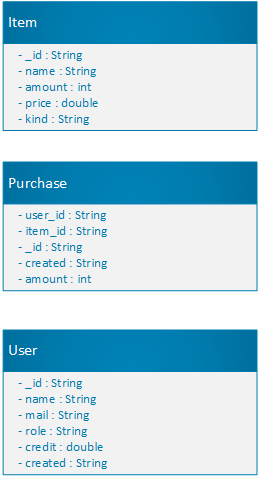
\includegraphics{datamodel.png}
			\caption{Datenmodell}
		\end{figure}
		
		
		\subsection{Frontend-Architektur} \label{architecture.frontend}
		
		\subsection{Backend-Architektur} \label{architecture.backend}
			\paragraph*{}
			Die Backend-Architektur besteht aus drei Ebenen. Die unterste Ebene bildet die Klasse \texttt{OkHttpConnection}, welche über das Interface \texttt{HttpConnection} implementiert ist. Die Klasse ist verantwortlich für den primitiven Netzwerkverkehr per HTTP mit beliebigen Inhalten. Es werden die HTTP-Methoden \texttt{GET}, \texttt{POST}, \texttt{PUT} und \texttt{DELETE} implementiert. Bei fehlerhaften Anfragen (HTTP-Code $\neq$ 2xx), sowie bei fehlerhaften URLs wird eine Exception geworfen.
			
			\paragraph*{}
			Auf der zweiten Ebene befinden sich die Klassen \texttt{KitchenConnection}, \texttt{LocalDataStore} und \texttt{JsonTranslator}.
			
			\begin{itemize}
				\item  \texttt{KitchenConnection} ist verantwortlich für die spezialisierte Kommunikation mit der bereitgestellten REST-API. Die Klasse enthält Attribute für die Basis-URL des REST-Servers, sowie für Schlüssel zur Erzeugung von Nutzern. Alle Funktionen der REST-API werden hier implementiert, indem jede Methode der Klasse einen Pfad der REST-API abdeckt. Die Funktionsnamen entsprechen der Spezifikation der REST-API.
				
				\item \texttt{LocalDataStore} ist verantwortlich für das Zwischenspeichern der User, Items und Purchases. Dies ermöglicht schnelleren Zugriff auf die jeweiligen Objekte.
				
				\item \texttt{JsonTranslator} ist verantwortlich für die bidirektionale Umwandlung zwischen Objekten des Datenmodells und JSON-Strings. Die verwendete Bibliothek für die Umwandlung ist Google's \texttt{GSON}.
			\end{itemize}
		
			\paragraph*{}
			Die Dritte Ebene beinhaltet nur die Klasse \texttt{KitchenManager}. Sie ist der Einstiegspunkte des Backend und stellt so alle Operationen zur Verfügung, welche die Oberfläche benötigt.
		
			\begin{figure}[!h]
				\centering
				\label{backendArchitecture}
				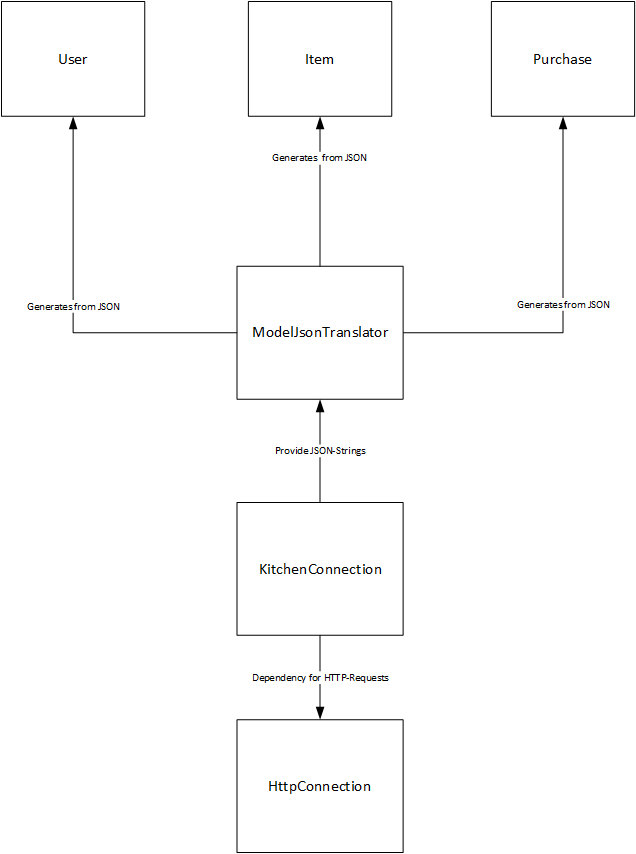
\includegraphics[scale=0.5]{./figures/classStructure.png}
				\caption{Backend Architektur}
			\end{figure}
	
	\section{Anhang: Build-Umgebung} \label{build}
	
	\section{Anhang: Bibliotheken} \label{bib}

	\section{Anhang: Tests} \label{tests}
	
\end{document}